\chapter{Item definition}
\label{ch:item_definition}

% Instructions:
% REQUIRED
% 
% Discuss these key points about the system:
% 
% What is the item in question, and what does the item do?
 
The item in question is the Lane Assitance system, with the purpose to assist
the driver in staying in the lane, and notifying the driver if a car is leaving
the lane.

% What are its two main functions? How do they work?

The Lane Assistance System has two functions:

\begin{enumerate}
  \item Lane departure warning
  \item Lane keeping assistance
\end{enumerate}

``The lane departure warning function shall apply an oscillating steering torque
to provide the driver a haptic feedback'': whenever a car is about to leave 
the lane where the car is currently driving, a steering wheel vibrates and 
alerts the driver about this situation.


``The lane keeping assistance function shall apply the steering torque when
active in order to stay in ego lane'': i.e. the lane keeping assistance 
steers the vehicle towards the center of the current driven lane.


 
% What subsystems are inside the item? 
The lane assistance system consists of the following sub-systems
(Fig.~\ref{fig:architecture}):

\begin{itemize}
  \item Camera sub-system;
  \item Electronic Power Steering sub-system;
  \item Car Display sub-system.
\end{itemize}


\begin{figure}[htbp]
\includegraphics[width=1.00\linewidth]{graphic_asset_2}
\caption{Lane assistance system architecture}
\label{fig:architecture}
\end{figure}

% Which subsystems are responsible for each function?
A camera sub-system is responsible for detecting position of the car w.r.t. 
to the center of the ego lane and w.r.t. to the road and sending a torque
request.

An electronic power steering ECU is responsible for receiving a torque
request and activating a motor providing torque request to the steering 
wheel. 

A car display sub-system is used to warn a driver about mal-function of the 
system.

% What are the boundaries of the item? 
The item boundaries are illustrated in Figure~\ref{fig:boundaries}:

\begin{figure}[htbp]
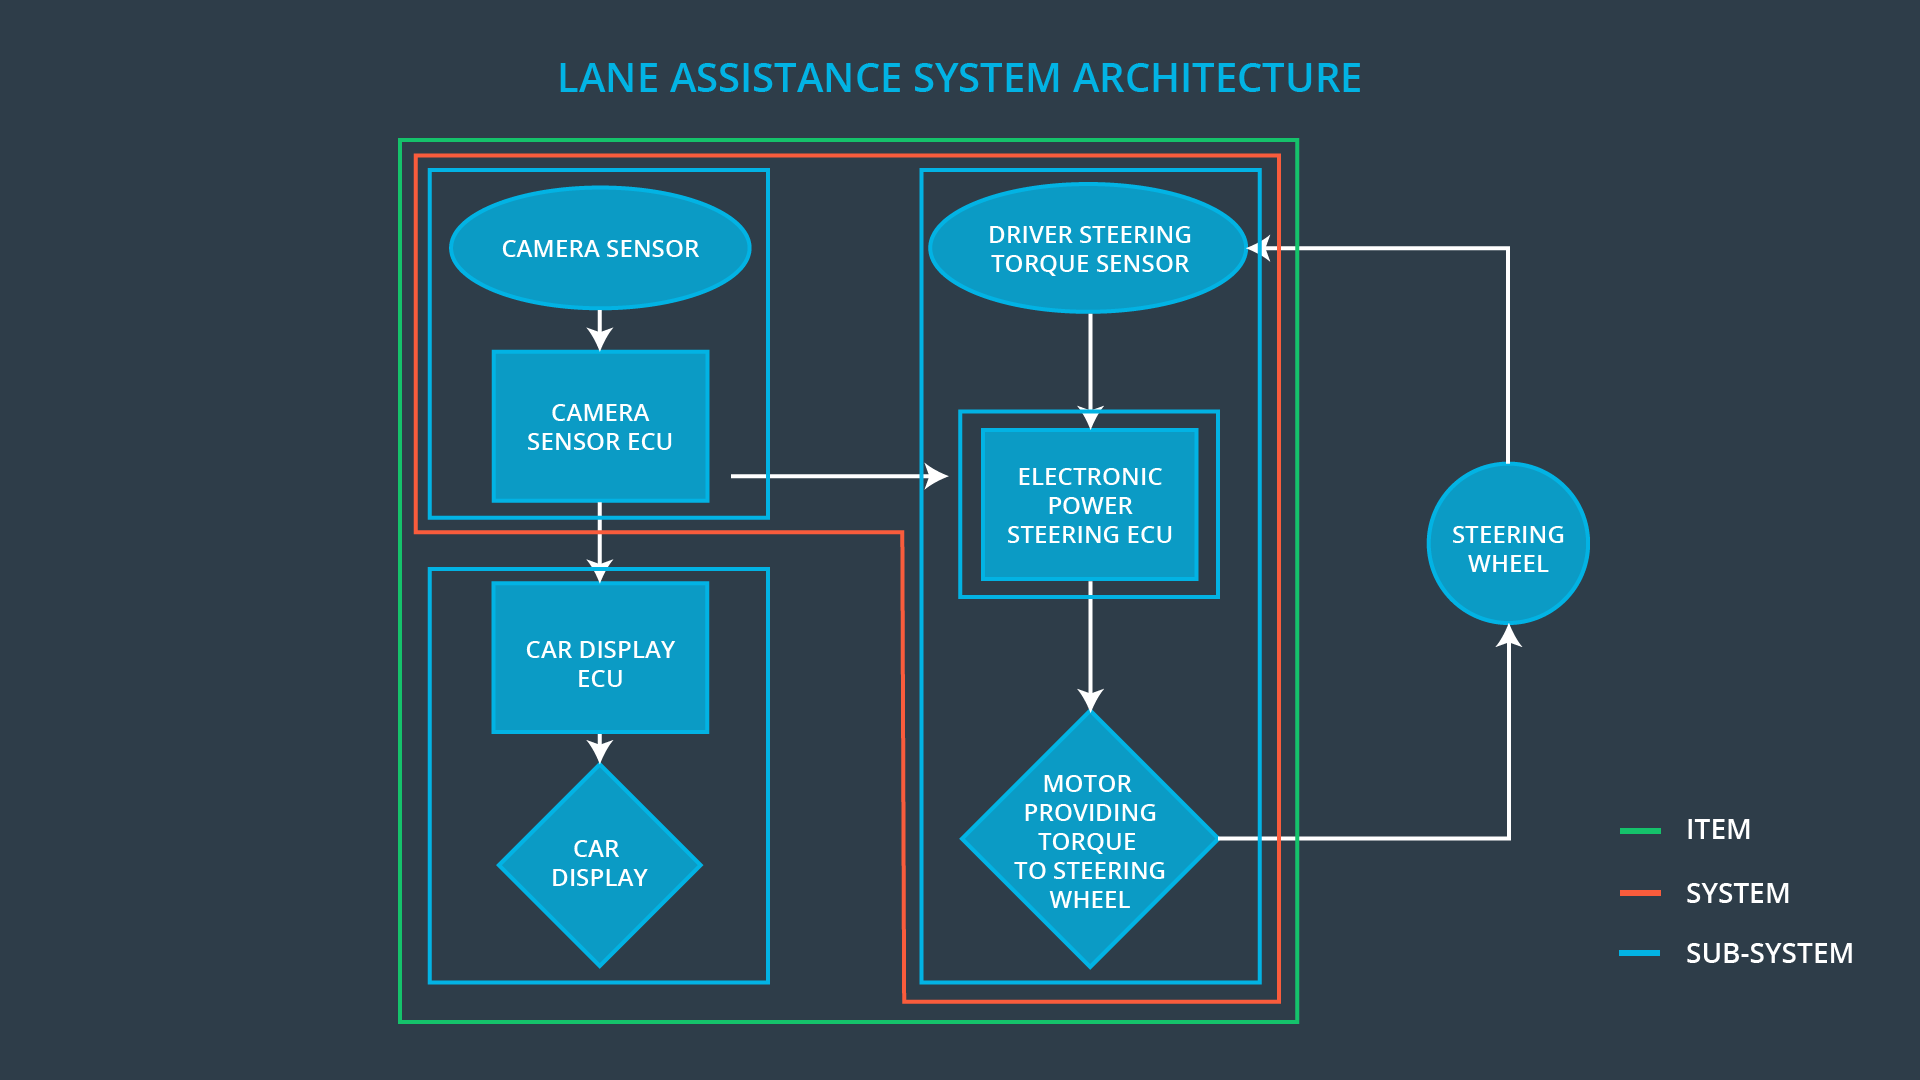
\includegraphics[width=1.00\linewidth]{02-advanced-driver-assistance-system-architecture-01}
\caption{Boundaries of the Lane assistance system and its sub-systems}
\label{fig:boundaries}
\end{figure}


% What elements or subsystems are outside of the item?

As seen from the Figure~\ref{fig:boundaries} the steering wheel is 
outside the Lane Assistance Item.
It is also implied that the engine, the breaking item are outside 
the Lane Assistance Item.

% OPTIONAL
% Optionally, include information about these points as well. These were not
% included in the lectures, but you might be able to find this information
% online:
% - Operational and Environmental Constraints. This could especially be limited
%   to camera performance; lane lines are difficult to detect in snow, fog, etc
% - Legal requirements in your country for lane assistance technology
% - National and International Standards Related to the Item
% - Records of previously known safety-related incidents or behavioral shortfalls

